\documentclass{beamer}

\usepackage{../packages/packages_mathalea}
\input{../competences/competences_latex.tex}
\usepackage{fontawesome}
\begin{document}

%%%%%%%%%%%%%%%%%%%%%%%%%%%%%%%%%%%%%%%%%%%%%%%%%%%%%%%%%%%%%%%%%%%%%%%%%%%%%%%
%%%%%%%%%%%%%%%%%%%%%%%%%%%%%%%%%%%%%%%%%%%%%%%%%%%%%%%%%%%%%%%%%%%%%%%%%%%%%%%
%%%%%%%%%%%%%%%%%%%%%%%%%%%%%%%%%%%%%%%%%%%%%%%%%%%%%%%%%%%%%%%%%%%%%%%%%%%%%%%

\begin{frame}{\GetCompetence{Fonc5} \\\GetCompetence{Fonc3}}
	% increment the counter
	\begin{itemize}
		\item<1->  Établir à l'aide de la calculatrice un tableau de valeur pour la fonction $x\mapsto -3x^2-\dfrac{1}{2}x+2$.
		\item<1-> Calculer la préimage de $-4$ par la fonction $f$. 
		\item<1-> Représenter graphiquement la droite $(d):y=-\dfrac{1}{2}x+2$.
	\end{itemize}

	\onslide<2->{{\bfseries Solution~:}}  
		\begin{itemize}
			\item<2-> Utiliser la calculatrice (c.f. vidéo).
			\item<2-> On résout l'équation $-3x^2-\dfrac{1}{2}x+2=-4$ et on obtient que la préimage de $-4$ par $f$ est $\left\{-\dfrac{3}{2}\,\;\,\dfrac{4}{3}\right\}$.
		\end{itemize}

\end{frame}
\begin{frame}
\begin{center}
	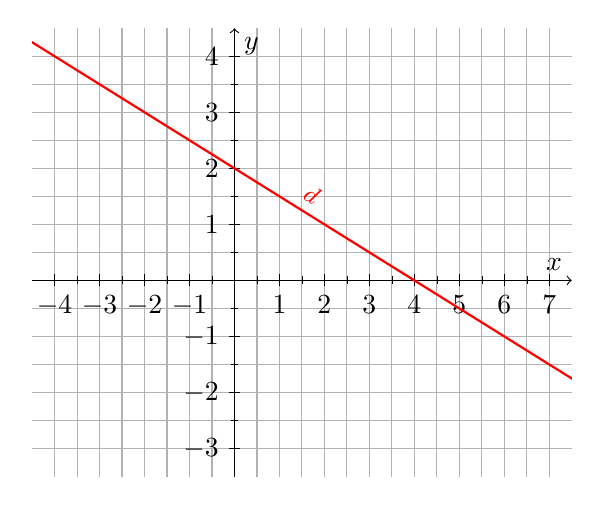
\begin{tikzpicture}[scale=1]
    % Define axis
    \begin{axis}[
        axis lines=middle,
        grid=both,
        minor tick num=1,
        xlabel={$x$},
        ylabel={$y$},
        xmin=-4.5, xmax=7.5,
        ymin=-3.5, ymax=4.5,
        xtick={-4,-3,-2,-1,0,1,2,3,4,5,6,7},
        ytick={-3,-2,-1,0,1,2,3,4},
        axis line style={->},
        tick style={black},
        label style={font=\bfseries},
        grid style={black!30}
    ]
        % Line d1
        \addplot[domain=-5:8, thick, red] { - 1/2*x+2} node[pos=0.5, above, sloped] {\small $d$};
    \end{axis}
\end{tikzpicture}
\end{center}
\end{frame}

\end{document}
